\section{28.10.2014 - Circuito per elettrocardiogramma (ECG)}

In questa esperienza ingegneristica costruiremo un circuito per effettuare un elettrocardiogramma (ECG).

\subsection*{Strumenti e materiali}

\begin{itemize} [noitemsep]
	\item Oscilloscopio Agilent DSO-X 2002A (bandwidth \SI{70}{\mega\hertz}, sample rate \num{2} GSa/s);
		\item Generatore di tensione continua Agilent E3631A (max $\pm \, \SI{25}{\volt}$ o $\pm \, \SI{6}{\volt}$);
		\item Multimetro Agilent 34410A a sei cifre e mezza;
		\item Due pile da \SI{9}{\volt};
		\item Amplificatori operazionali OP07;
		\item Un integrato AD622 e un ISO124;
		\item Resistenze e capacità di vari valori;
		\item Breadboard e cablaggi vari;
		\item Paziente (umano).
\end{itemize}

\begin{wrapfigure}[20]{r}{0.24\textwidth}
\centering
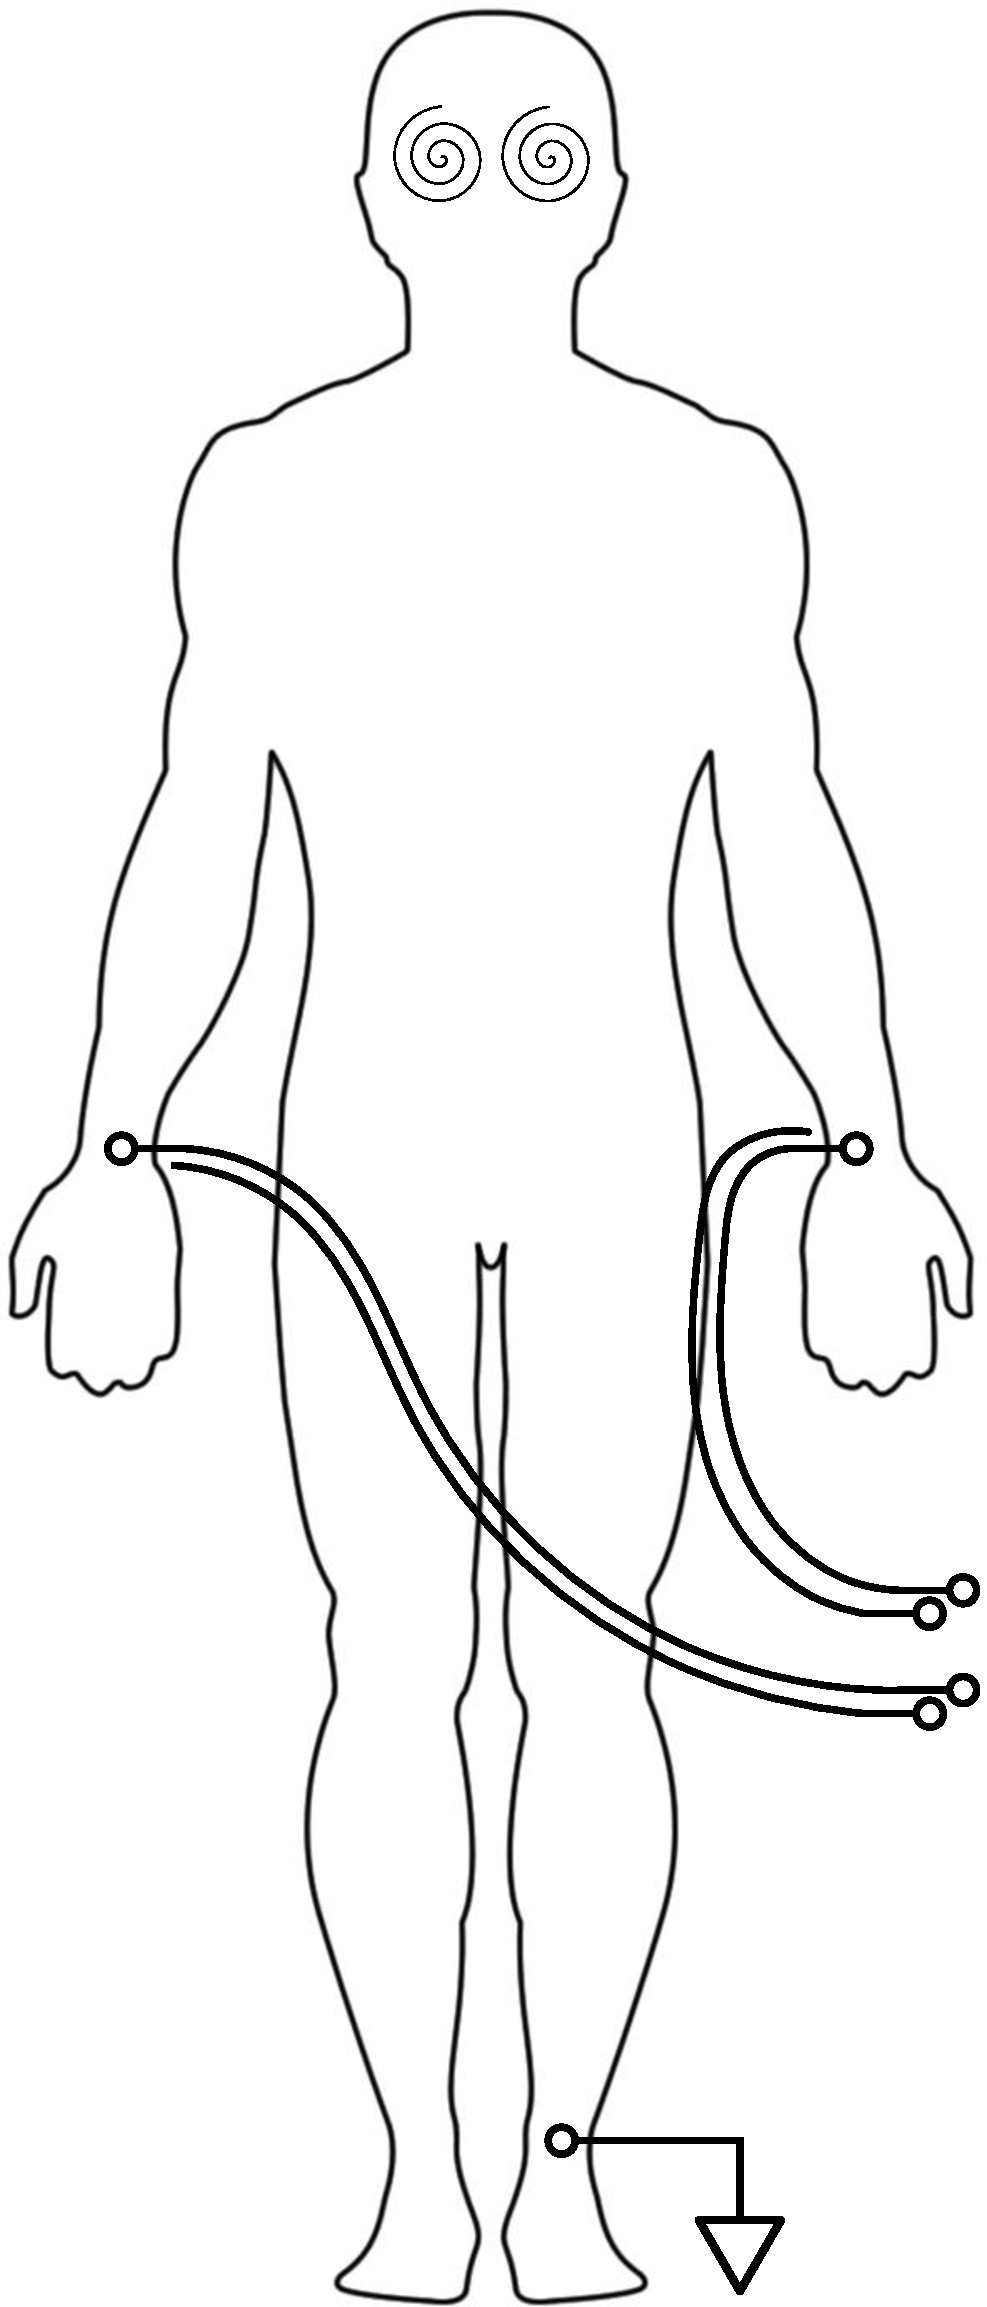
\includegraphics[width=.18\textwidth]{../E07/latex/human.pdf}
\caption{Connessioni al corpo poco umano di uno degli sperimentatori.}
\label{fig7:human}
\end{wrapfigure}
